\documentclass[UTF8,a4paper,12pt,fontset=fandol]{ctexart}
\usepackage[top=2.5cm,bottom=2.5cm,left=2.5cm,right=2.5cm]{geometry}
\usepackage{amsmath,amssymb,bm}
\usepackage{graphicx}
\usepackage{booktabs}
\usepackage{float}
\usepackage{siunitx}
\usepackage{enumitem}
\usepackage{hyperref}
\hypersetup{colorlinks=true,linkcolor=black,citecolor=black,urlcolor=blue}

\title{语音信号处理实验八报告}
\author{胡伟毅 12313505\quad 安文博 12310403}
\date{2026 年 4 月 24 日}

\begin{document}
\maketitle

\section{实验目的与完成情况}

本实验围绕语音参数估计中的平滑处理和基音检测展开，主要目的包括：掌握中值平滑及组合平滑在语音参数轨迹中的作用；实现并比较基于改进自相关和实倒谱的基音周期估计算法；观察带通预处理、置信度阈值和可靠区扩展对基音轨迹连续性的影响。

本报告对应完成的程序文件包括主脚本、三类平滑器和两类基音检测器。实验输出包括三组结果图、两组过程图以及 \texttt{out\_autoc.mat}、\texttt{out\_cepstrum.mat}。其中 Problem 2 的全带重采样语音和带通滤波语音也作为试听比较对象，用于判断滤波是否明显削弱直流、低频工频干扰和高频噪声。核心代码文件如下：
\begin{itemize}[noitemsep]
    \item \texttt{lab8\_main.m}
    \item \texttt{MedianSmoother.m}、\texttt{LinearSmoother.m}、\texttt{CombinationSmoother.m}
    \item \texttt{PitchDetector\_Autocorrelation.m}、\texttt{PitchDetector\_Cepstrum.m}
\end{itemize}

\section{Problem 1：短时过零率与平滑器比较}

\subsection{方法}

对 \texttt{test\_16k.wav} 进行短时过零率估计。实验采用 \SI{10}{ms} 帧长和 \SI{5}{ms} 帧移。第 $m$ 帧的过零率定义为
\begin{equation}
    \mathrm{ZCR}(m)=\frac{1}{2}\sum_{n=1}^{N-1}\left|\operatorname{sgn}(x_m[n+1])-\operatorname{sgn}(x_m[n])\right|,
\end{equation}
其中 $x_m[n]$ 表示第 $m$ 帧语音，$N$ 表示一帧中的采样点数。这里保留过零次数形式，便于直接观察每个 \SI{10}{ms} 区间内的变化幅度。

得到原始过零率序列后，分别使用三类平滑器：
\begin{enumerate}[label=(\arabic*)]
    \item 线性平滑：用长度 $L=41$ 的低通 FIR 滤波器平滑过零率轮廓，并补偿线性相位群延迟；
    \item 中值平滑：先进行 7 点中值平滑，再进行 5 点中值平滑，用于抑制局部毛刺；
    \item 组合平滑：先提取平滑主趋势，再对残差平滑后叠加，形式为
    \begin{equation}
        y[n]=S\{x[n]\}+S\{x[n]-S\{x[n]\}\},
    \end{equation}
    其中 $S\{\cdot\}$ 表示“中值平滑 + 线性平滑”的组合操作。
\end{enumerate}

\subsection{结果与分析}

\begin{figure}[H]
    \centering
    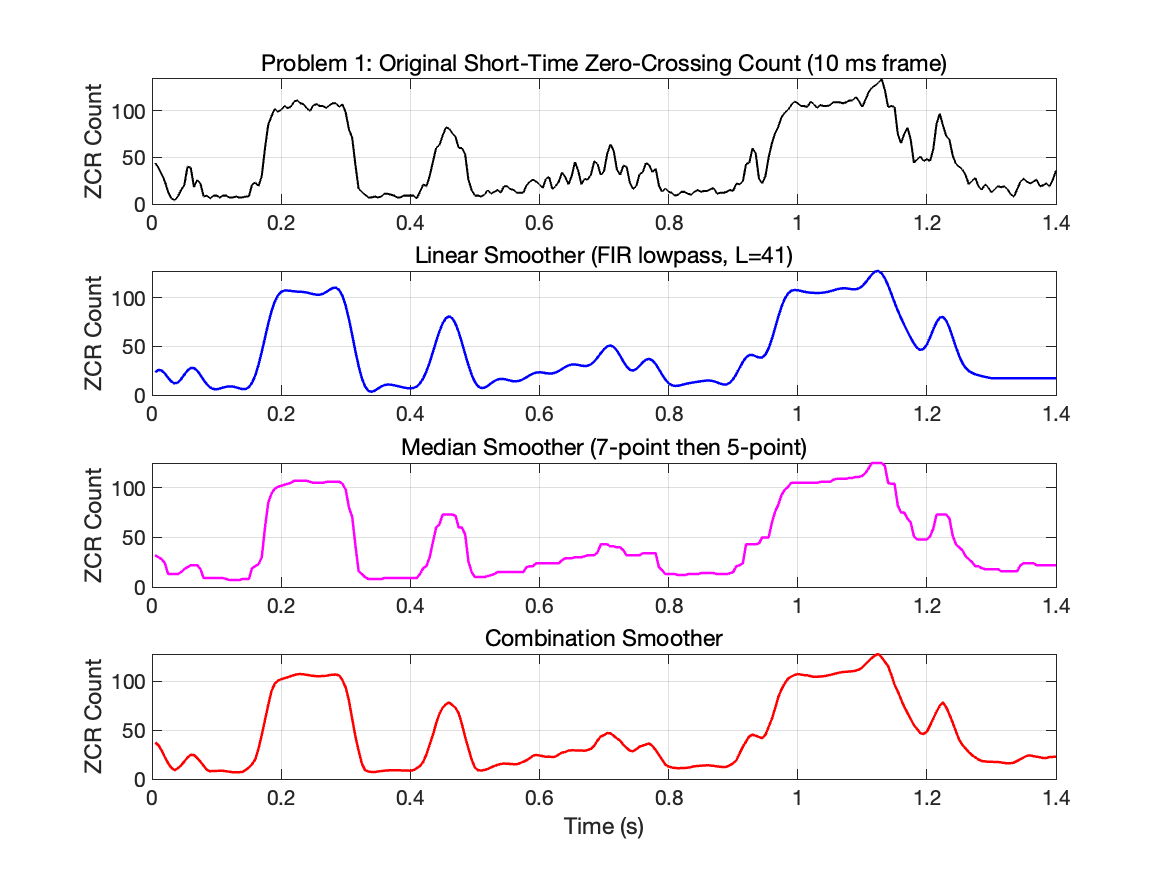
\includegraphics[width=0.96\textwidth]{problem1_zcr_smoothing.png}
    \caption{短时过零率原始曲线及三类平滑结果}
\end{figure}

\begin{table}[H]
    \centering
    \caption{Problem 1 平滑效果指标}
    \begin{tabular}{lcc}
        \toprule
        曲线 & 序列标准差 & 一阶差分标准差 \\
        \midrule
        原始 ZCR & 37.6623 & 8.3837 \\
        线性平滑 & 37.3306 & 4.8228 \\
        中值平滑 & 36.9726 & 5.7354 \\
        组合平滑 & 37.0091 & 4.7034 \\
        \bottomrule
    \end{tabular}
\end{table}

从图中可以看出，原始过零率曲线存在明显的高频起伏。三类平滑方法均能降低局部抖动，但保留语音段和非语音段之间的整体变化趋势。线性平滑的轮廓更连续，中值平滑对尖峰抑制更直接，组合平滑兼顾主趋势和残差修正，其一阶差分标准差最低，说明局部抖动被压制得最充分。因此在本数据上，组合平滑最适合用于保留过零率主要轮廓并减少毛刺。

\section{Problem 2：基于改进自相关的基音检测}

\subsection{方法}

本部分以 \texttt{s6.wav} 为输入，实现基于改进自相关的基音周期检测。处理流程如下：
\begin{enumerate}[label=(\arabic*)]
    \item 将输入语音重采样到 $f_{s,out}=\SI{10}{kHz}$；
    \item 设计长度为 301 的 FIR 带通滤波器，频带设置用于抑制直流、低频干扰和 \SI{900}{Hz} 以上的高频成分；
    \item 同时保留全带重采样语音和带通滤波语音，分别用于后续基音检测和试听比较；
    \item 采用 $L=400$、$R=100$ 分帧，即帧长约 \SI{40}{ms}、帧移约 \SI{10}{ms}；
    \item 按男性说话人设定搜索范围
    \begin{equation}
        \mathrm{pdlow}=\left\lceil\frac{f_{s,out}}{200}\right\rceil=50,
        \quad
        \mathrm{pdhigh}=\left\lfloor\frac{f_{s,out}}{75}\right\rfloor=133;
    \end{equation}
    \item 对每帧计算延迟相关，在 $[\mathrm{pdlow},\mathrm{pdhigh}]$ 内寻找最大峰值，将峰值位置作为候选基音周期，将峰值大小作为置信度；
    \item 对置信度取 $\log_{10}$，用 $0.75\times\max$ 作为阈值，低于阈值的帧将基音周期置零；
    \item 对基音周期和置信度序列分别做 5 点中值平滑。
\end{enumerate}

第 $i$ 帧中使用的改进相关可写为
\begin{equation}
    c_i(\tau)=\sum_{n=0}^{L-1}x_i[n]x_i[n+\tau],
    \quad \tau\in[\mathrm{pdlow},\mathrm{pdhigh}].
\end{equation}
若 $c_i(\tau)$ 的最大值明显大于其他延迟处的相关值，则该帧更可能包含稳定周期结构。

\subsection{结果与分析}

\begin{figure}[H]
    \centering
    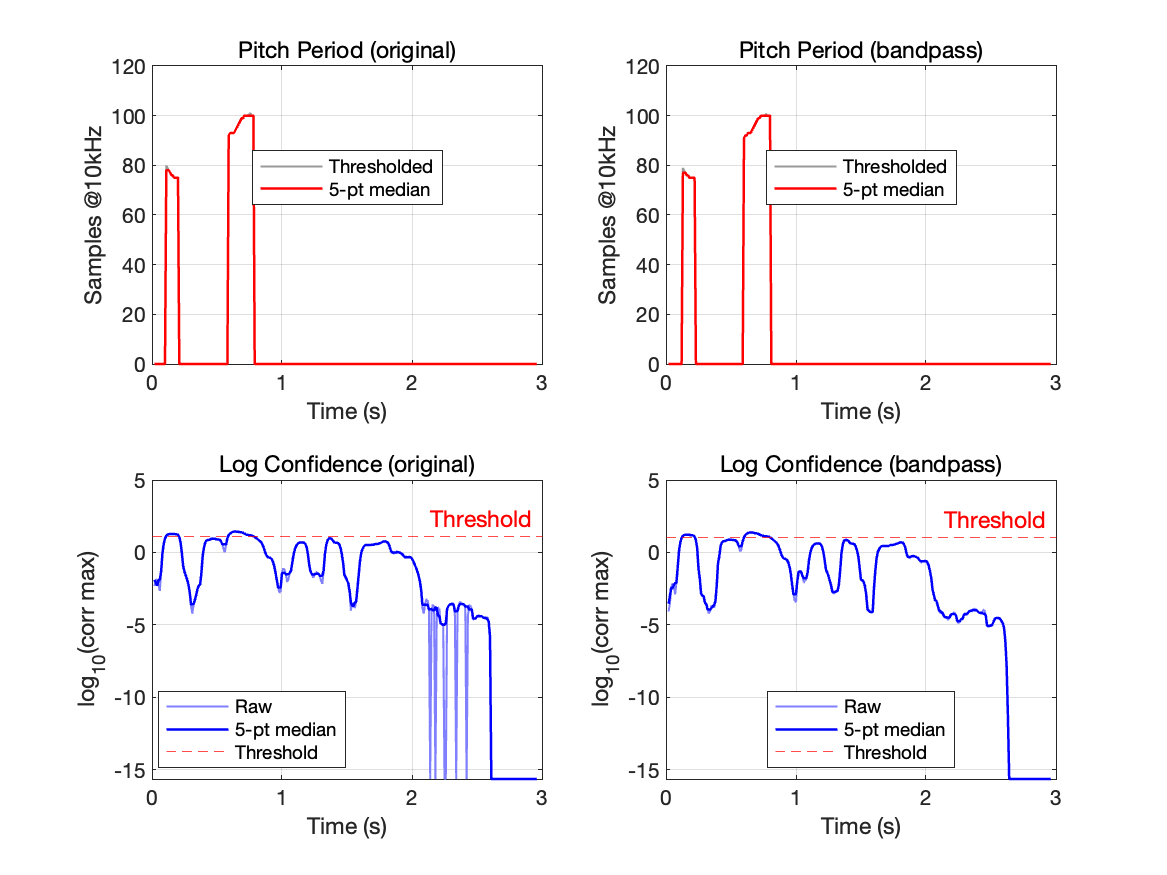
\includegraphics[width=0.95\textwidth]{problem2_autoc_pitch.png}
    \caption{改进自相关法得到的基音周期与对数置信度}
\end{figure}

\begin{table}[H]
    \centering
    \caption{Problem 2 自相关法统计结果}
    \resizebox{\textwidth}{!}{
    \begin{tabular}{lcccccc}
        \toprule
        信号 & 帧数 & 非零基音帧数 & 占比 & 阈值 & 平均周期(样本) & 平均基频(Hz) \\
        \midrule
        原始语音（s6） & 295 & 30 & 0.1017 & 1.0846 & 90.17 & 110.91 \\
        带通语音（s6） & 295 & 31 & 0.1051 & 1.0313 & 90.00 & 111.11 \\
        \bottomrule
    \end{tabular}}
\end{table}

从统计结果看，原始语音和带通语音的平均基音周期分别约为 90.17 和 90.00 个 \SI{10}{kHz} 采样点，对应平均基频约为 \SI{111}{Hz}。两条基音轨迹非常接近，说明该语音片段的主周期较稳定，自相关方法能够在两种预处理条件下给出一致估计。

带通滤波后，非零基音帧数从 30 增加到 31，阈值略有降低。这表明滤波对少数边缘帧的置信度有一定帮助，但总体改善幅度不大。试听比较中，全带语音保留了更多背景和宽带细节，带通语音听感更集中于浊音周期相关频段，低频轰声和高频细节有所削弱；这种处理有利于自相关峰更加突出，但也可能使部分非周期语音信息被削弱。

\section{Problem 3：基于实倒谱的基音检测}

\subsection{方法}

本部分使用实倒谱估计基音周期。输入语音仍为 \texttt{s6.wav}，同样比较全带重采样语音和带通滤波语音。每帧使用 $L=400$，帧移 $R=100$，FFT 点数设为 \texttt{nfft}=4000。实倒谱定义为
\begin{equation}
    c[n]=\mathcal{F}^{-1}\left\{\log\left|X[k]\right|\right\}.
\end{equation}

对男性说话人，倒频率搜索范围设为
\begin{equation}
    n_{low}=40,\quad n_{high}=167.
\end{equation}
该范围大致对应常见男性基频的周期范围。对每一帧，在此区间内寻找主峰 $p_1$ 及其位置 $pd_1$。随后将主峰附近若干点置零，再寻找次峰 $p_2$ 及其位置 $pd_2$。若
\begin{equation}
    \frac{p_1}{p_2}\ge p_{thr1}=4,
\end{equation}
则该帧被视为可靠种子帧。之后以可靠帧为边界向相邻帧扩展：如果相邻帧的主峰或次峰周期与当前边界周期的相对偏差不超过 $10\%$，则将该帧纳入可靠区。最后对扩展后的基音周期曲线和置信度曲线分别做 5 点中值平滑。

\subsection{结果与分析}

\begin{figure}[H]
    \centering
    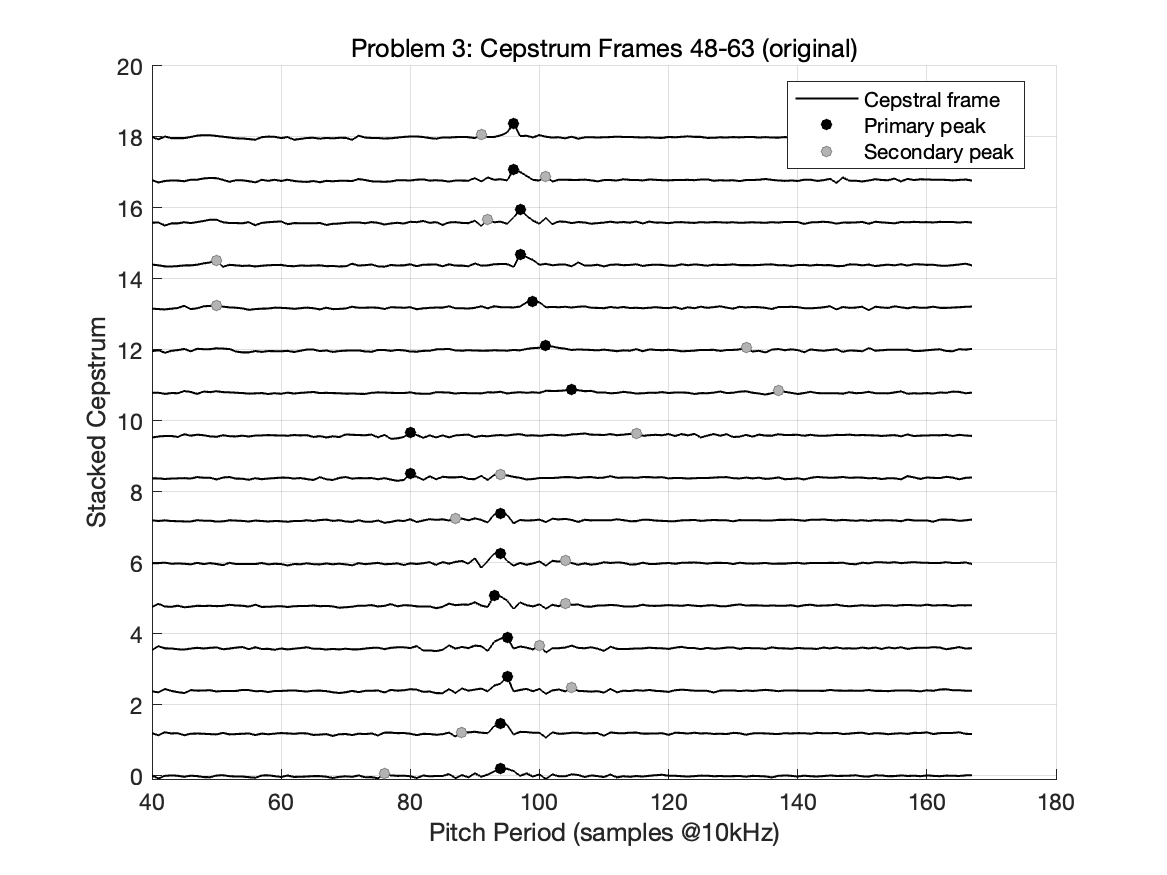
\includegraphics[width=0.92\textwidth]{problem3_cepstrum_waterfall.png}
    \caption{倒谱帧瀑布图及主峰、次峰标注}
\end{figure}

\begin{figure}[H]
    \centering
    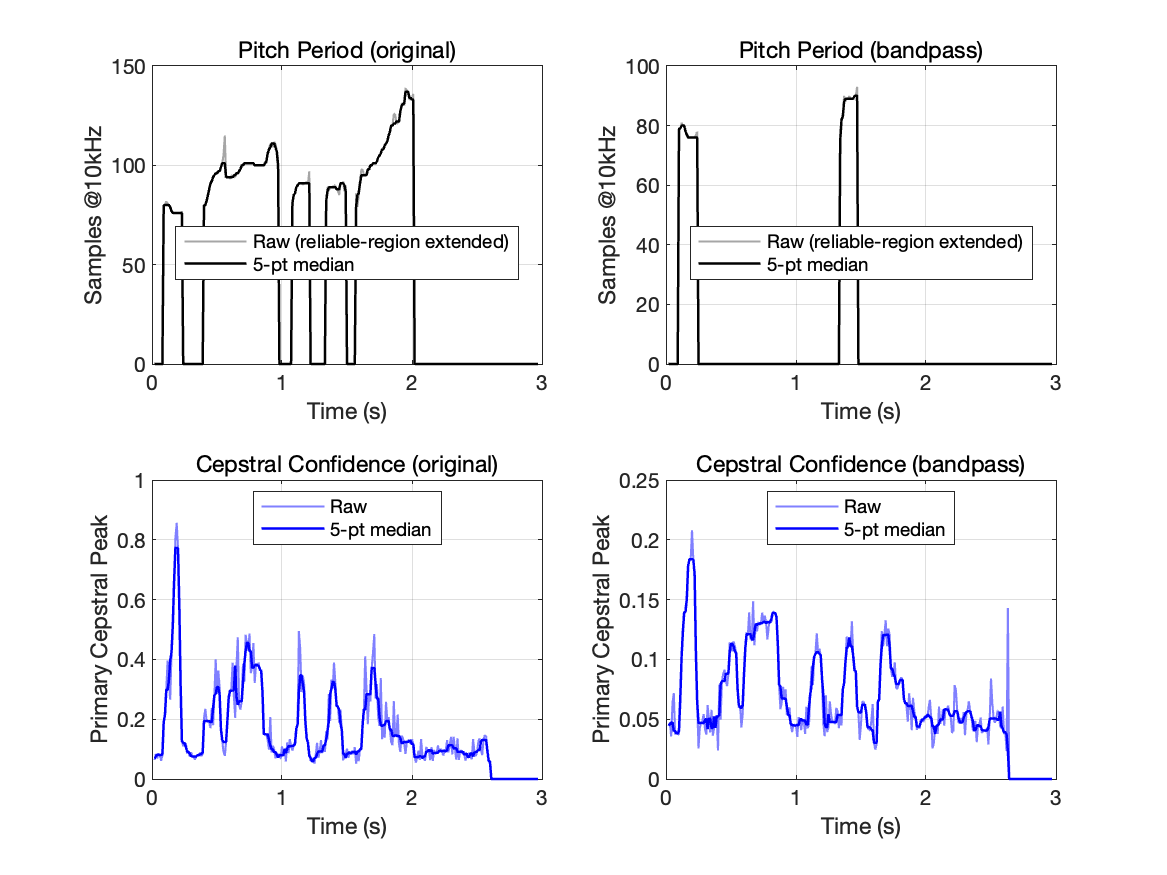
\includegraphics[width=0.95\textwidth]{problem3_cepstrum_pitch.png}
    \caption{实倒谱法得到的基音周期与倒谱峰值置信度}
\end{figure}

\begin{table}[H]
    \centering
    \caption{Problem 3 实倒谱法统计结果}
    \resizebox{\textwidth}{!}{
    \begin{tabular}{lcccccc}
        \toprule
        信号 & 帧数 & 非零基音帧数 & 占比 & 可靠种子帧数 & 平均周期(样本) & 平均基频(Hz) \\
        \midrule
        原始语音（s6） & 296 & 148 & 0.5000 & 58 & 98.34 & 101.68 \\
        带通语音（s6） & 296 & 29 & 0.0980 & 7 & 82.14 & 121.75 \\
        \bottomrule
    \end{tabular}}
\end{table}

倒谱法在原始语音上形成了较长的连续有效区段，共有 58 个可靠种子帧，扩展和平滑后得到 148 个非零基音帧。其平均基频约为 \SI{101.68}{Hz}，与自相关法的结果同属男性语音常见范围，但数值略低，说明两种算法在峰值选择和可靠区定义上存在差异。

带通语音在倒谱法下的有效帧明显减少，可靠种子帧仅有 7 个，扩展后非零帧数为 29。这说明固定的主峰/次峰比阈值对预处理方式较敏感。带通滤波虽然能突出周期相关成分，但也会改变谱包络与倒谱峰之间的相对关系，使部分帧的主峰优势下降。因此，倒谱法若用于不同滤波条件，最好进一步采用自适应阈值或结合能量、过零率等辅助判据。

\section{综合讨论}

\subsection{平滑方法的作用}

无论是短时过零率还是基音周期轨迹，原始估计值都容易受到局部噪声、边界帧和短时非平稳性的影响。中值平滑能够有效去除孤立异常点，线性平滑能够降低快速抖动，组合平滑则进一步兼顾趋势保持和残差修正。在本实验中，组合平滑对 ZCR 的一阶差分标准差降低最明显；在基音检测中，5 点中值平滑使基音轨迹更加连续，减少了孤立误检帧的视觉干扰。

\subsection{两种基音检测方法比较}

自相关法直接利用时域周期性，结果较稳定，对带通预处理不太敏感；本实验中原始语音和带通语音的平均基频几乎一致。实倒谱法通过倒频率域峰值反映基音周期，能够给出较清晰的峰值结构和可靠区，但对谱包络、滤波方式以及主峰/次峰比阈值更敏感。两者相比，自相关法更适合作为稳健基线，倒谱法更适合结合峰值可视化分析周期结构。

\subsection{误差来源}

实验中可能的误差来源包括：重采样和滤波引入的边界效应；静音帧或清辅音帧中缺少稳定周期导致误检；固定阈值无法适应所有语音段；基音周期搜索范围由性别先验确定，若实际说话人基频偏离范围边界，可能造成候选周期偏差。后续可引入端点检测、自适应阈值和动态规划连续性约束进一步提升轨迹稳定性。

\section{结论}

本实验完整实现了短时过零率平滑、改进自相关基音检测和实倒谱基音检测三项任务。主要结论如下：
\begin{enumerate}[label=(\arabic*)]
    \item 对短时过零率而言，线性平滑、中值平滑和组合平滑都能减少局部抖动，其中组合平滑的一阶差分标准差最低，整体效果最好；
    \item 改进自相关法在原始语音和带通语音上均得到约 \SI{111}{Hz} 的平均基频，说明其对当前语料具有较好的稳定性；
    \item 实倒谱法能够通过主峰/次峰比和可靠区扩展得到基音轨迹，但对带通滤波和固定阈值更敏感；
    \item 平滑和置信度控制是语音参数估计中非常重要的后处理环节，可以显著改善参数轨迹的可读性和可靠性。
\end{enumerate}

综上，本次实验达到了课件中关于平滑处理、自相关基音检测和倒谱基音检测的要求，并通过图形、统计量和听感比较对不同处理策略进行了验证。

\end{document}
